\section{Finite state machines}
% ========================================
% 
% ========================================
\begin{frame}{Finite State Machines}{}
  \begin{itemize}
    \item A \ac{FSM} is an abstract device used to model, monitor and save the status of a system.
    \item The status of a system may be known by inspecting a \emph{state variable}, simply referred to as \alertblue{state}.
    \item Moreover, the immediate future status of a system may be known by inspecting both the current \alertblue{state} and the current \alertblue{inputs} of the system.
    \item In digital electronics, \acp{FSM} are deterministic synchronous models which are commonly used as an essential part of control units.
    \item \acp{FSM} are classified in two main categories according to their outputs.
    \begin{itemize}
      \item Moore.
      \item Mealy.
    \end{itemize}
  \end{itemize}
\end{frame}

% ========================================
% 
% ========================================
\begin{frame}{Finite State Machine}{}
\begin{figure}
  \centering
  \begin{subfigure}{\textwidth}
    \centering
     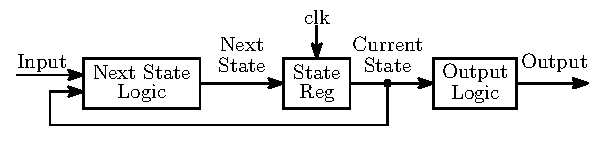
\includegraphics[width=\textwidth]{FSM_Moore}
     \caption{Moore \ac{FSM}.}
     \label{Figure:FSM_Moore}
  \end{subfigure}
  \\
  \begin{subfigure}{\textwidth}
    \centering
    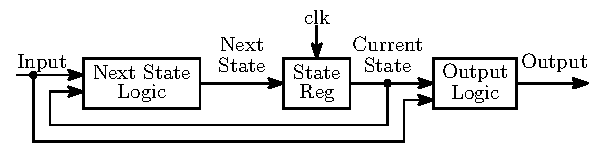
\includegraphics[width=\textwidth]{FSM_Mealy}
    \caption{Mealy \ac{FSM}.}
    \label{Figure:FSM_Mealy}
  \end{subfigure}
  \vspace{-12pt}
  \caption{\acp{FSM}}
  \label{Figure:FSMs}
\end{figure}
\end{frame}

% ========================================
% 
% ========================================
\begin{frame}{Finite State Machines}{}
  \begin{itemize}
    \item \acp{FSM} may be represented by state diagrams.
    \begin{figure}
      \centering
      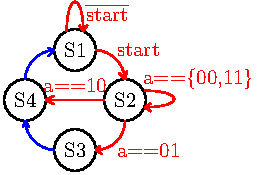
\includegraphics[scale=2.0]{FSM_transitions}
       \caption{Transitions in state diagrams.}
       \label{Figure:FSM_transitions}
    \end{figure}
  \end{itemize}
\end{frame}

% ========================================
% 
% ========================================
\begin{frame}{Finite State Machines}{}
  \begin{itemize}
    \item Moore state diagram.
    \begin{figure}
      \centering
      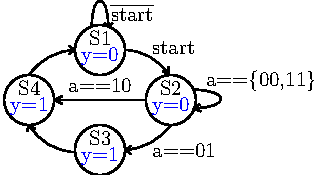
\includegraphics[scale=2.0]{FSM_Moore_diagram}
       \caption{Moore state diagram.}
       \label{Figure:FSM_Moore_diagram}
    \end{figure}
  \end{itemize}
\end{frame}

% ========================================
% 
% ========================================
\begin{frame}{Finite State Machines}{}
  \begin{itemize}
    \item Mealy state diagram.
    \begin{figure}
      \centering
      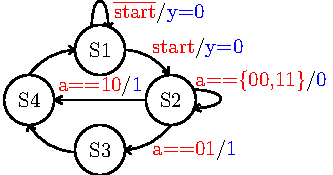
\includegraphics[scale=2.0]{FSM_Mealy_diagram}
       \caption{Mealy state diagram.}
       \label{Figure:FSM_Mealy_diagram}
    \end{figure}
  \end{itemize}
\end{frame}

% ========================================
% 
% ========================================
\begin{frame}{Finite State Machines}{}
  \begin{itemize}
    \item State diagrams are useful with state machines with relatively few number of states.
    \item State diagrams might be difficult to understand if a system has
    \begin{itemize}
      \item A large number of transitions.
      \item A large number of outputs.
    \end{itemize}
    \item \ac{ASM} charts might be useful in these conditions.
    \begin{itemize}
     \item They are diagrams similar to flow charts.
    \end{itemize}
  \end{itemize}
\end{frame}
 
% ========================================
% 
% ========================================
\begin{frame}{}{}
\begin{figure}
\begin{minipage}[b]{0.5\linewidth}
  \begin{itemize}
    \item \ac{ASM} charts consist of three main components.
    \begin{itemize}
      \item \alertblue{State boxes.} Represented with a rectangular box,  contain the name of the state and an output list for the case of Moore outputs.
      \item \alertblue{Decision boxes.} Represented with a diamond-shaped box.
      \item \alertblue{Conditional boxes.} Represented with oval boxes, represent conditional output for the case of Mealy outputs.
    \end{itemize}
  \end{itemize}
\end{minipage}
%
\begin{minipage}[b]{0.49\linewidth}
\centering
  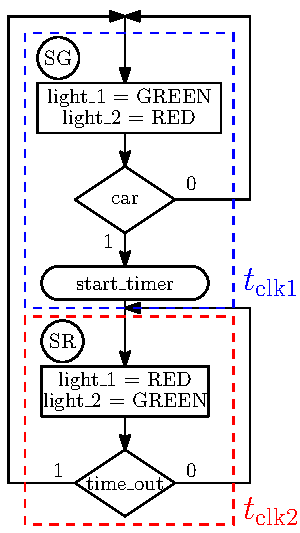
\includegraphics[scale=0.9]{ASM_chart}
  \vspace{-4pt}
  \caption{\ac{ASM} chart example.}
  \label{Figure:ASM_chart}
\end{minipage}
\end{figure}
\end{frame}

% ========================================
% 
% ========================================
\begin{frame}{ASM conditional output}{}
  \begin{figure}
  \centering
  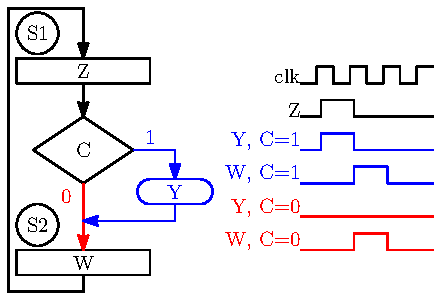
\includegraphics[scale=1.3]{ASM_chart_conditional}
  \vspace{-4pt}
  \caption{\ac{ASM} conditional output.}
  \label{Figure:ASM_conditional}
  \end{figure}
\end{frame}


% ========================================
% 
% ========================================
\begin{frame}{ASM unconditional output}{}
  \begin{figure}
  \centering
  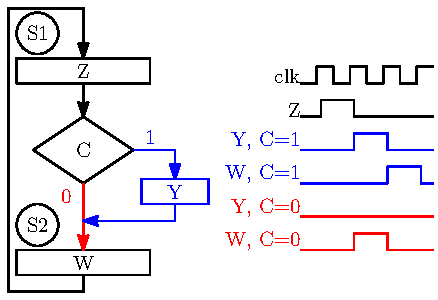
\includegraphics[scale=1.3]{ASM_chart_unconditional}
  \vspace{-4pt}
  \caption{\ac{ASM} unconditional output.}
  \label{Figure:ASM_unconditional}
  \end{figure}
\end{frame}